%!TEX root = project.tex

\chapter*{About this project}
\paragraph{Abstract}
The aim of this project was to create an application for the purpose of general election forecasting in an Irish setting. This process involved compiling a population database, using descriptive and inferential statistics and creating user-friendly interactive maps of Ireland. It was created using a 
combination of the following technologies: Neo4j, Python, Python Flask web framework and d3.JS. Data was extracted from the Central Statistics Office (CSO) and sorted using Python Pandas to be stored on Neo4j. The database consists of the population of the Republic of Ireland, including the entire electorate as well as potential future electorate members who are over the age of 18 and eligible to register. Data analysis was performed using both general probability and the d’Hondt method. The aim was to investigate how the results of the most recent election in Ireland (i.e. 2016) could be predicted using a combination of known demographic information as well as relevant polling data. The front-end of the project has been designed with two main views for illustrating the results. These maps are interactive and the user has a choice of two viewing options: 1) A view of two maps with one data panel, which displays information either regarding the predictions or the actual results depending on which map is interacted with, or 2) A view of one map with two panels of data, such that both the predictions and the results can be illustrated at the same time per county interacted with.

\paragraph{Authors}
The author of this project is Eamon McNicholas, a final year student of the BSc in Computing in Software Development Honours degree. 




\chapter{Introduction}

Since the advent of elections for choosing who represents us on a local, national or international scale, the forecasting of these elections has become of interest to a significant portion of the voting population. Where predictions are concerned, there are also huge monetary sums at stake for polling firms, news companies and gambling markets alike. For the majority of  people, polling of the electorate is the most well known of the election forecasting techniques commonly used. Generally,  the average of the latest polls is the most extensively accepted best indicator of the probable results of an election ~\cite{stegmaier}.

However, in two of the biggest voting events of the last year, the polls from major news firms and polling organisations were way off target ~\cite{ukbusinsider}.
In the UK, the referendum for choosing to stay or leave the European Union result went against the outcome predicted by the majority of major UK pollsters~\cite{bbcnews}.
In what was probably the most popular election in the world, the 2016 US presidential election surprised almost everyone when Donald Trump bet Hilary Clinton. A renowned statistical analyst, Nate Silver, created Fivethirtyeight.com, which is one of the most popular event prediction websites in the world. He gave Trump more of a chance of winning (35 percent) than anyone else, but his prediction was still wide off of the mark based on the actual results~\cite{natesilver}.

Other options for forecasting come in the form of creating various models of voting behaviour and regression models of previous elections in order to predict the results of future elections. The voting behaviour models take into account predictors (i.e. phenomena that can vary at any time) such as promised changes in tax rates or the creation of jobs in a area ~\cite{stegmaier}. This type of model can be useful for local elections[1]. Regression models such as a Bayesian forecasting model that take into account polling data as well as data from previous elections are also becoming an increasingly popular means for election forecasting, especially with the recent advent of more easily accessible data on the internet~\cite{rigdon}.

In this paper I will describe in detail my process for creating an election forecasting application, the challenges that I encountered as well as the research I conducted on the various areas of election forecasting.  I will then discuss how I translated this theory into practice by designing and implementing the ideas acquired from my research. To conclude, I will discuss the outcomes of my project, highlight any lessons learned along with my proposed recommendations for further research.

\chapter{Context}

\section{Scope and Context}
The purpose of this project is to develop an application that can be used for predicting the results of a general election in Ireland. Someone with a background in political science or data analytics could use this application with a model they have developed for election predictions. A database will be created which consists of the population in the Republic of Ireland who are eligible to register to vote or who are already registered to vote. By including the section of the population who are eligible to register to vote, but who have not actually done so, this allows for dramatic changes in the electorate to be accounted for. The database population will be categorized according to a number of relevant demographic characteristics in this context, including  social class, age-range, gender and martial status. Furthermore, the subsection of the population who live in counties with more than one constituency will also be taken into consideration as another relevant characteristic. 

The application will have a front end that consists of a web page with two interactive maps of the republic of Ireland. The first map will have display the predicted results and the second map will display the actual results. The prediction model being using in this application will be my own interpretation of how this software can be used.  It will be partially based on the model used by an Irish political analyst, Dr. Adrian Kavanagh, who specializes in this area ~\cite{adrian}.It will be the outcome of calculating the general probability of the results for each constituency by combining polling data and historical averages and then using the d’hondt method to assign seats to each party~\cite{adrian}.

\section{Objectives}
My main objective in this project was to create a full stack web application for election forecasting. This then generated the following secondary objectives:
\begin{itemize}
	\item To create a reasonably accurate database of the republic of Ireland's population who are eligible to vote as well as including the population who are eligible to register to vote.
	\item To create a model for predicting the general election results of a previous election so that it would be possible to compare the predicted and actual results. This would help create a benchmark against which the accuracy of my predictor model could then be compared.
\end{itemize}

However, as I became more familiar with the research regarding election forecasting, it became apparent that the process of creating a truly comprehensive statistical model would be beyond the scope of this project.  Subsequently, I then narrowed the focus of my secondary objectives to illustrating a basic example of how this type of model could be designed and implemented in practice. 

My final original objective had been to create an interactive map of Ireland which would allow the user to hover over each constituency to compare the actual results with those predicted.  However, I  found that it was much less complicated in practice to design two maps of Ireland where the counties were interactive, and the actual or the predicted results would be displayed depending on which map was clicked. 

\section{Links and Section Preview}
\begin{itemize}
	\item https://github.com/DevEMCN/Irish-Election-Forecasting---FYP
	\item https://github.com/DevEMCN/final-year-project-template
\end{itemize}
\subsection{Methodology}
This section will cover the way I approached and planned out how I was going to design this project, along with the methods used for data extraction. 
\subsection{Technology Review}
This section will review the technologies that were used in the development process. It will illustrate how the best fit development environment for the project was researched and how these tools were used to implement the project.
\subsection{System Design}
In this chapter, I will provide a comprehensive summary of the system architecture, including relevant illustrative diagrams and screenshots. 
\subsection{System Evaluation}
In this section, I will analyse my system design in terms of robustness and performance. I will also highlight any limitations of my design which became clearer to me towards the end of the project. 

\chapter{Methodology}
\paragraph{}
The following section will describe the methodologies and development approach used to design this project. It is divided into two main parts: 1) Research and 2) Development approach. The research section will also be further subdivided into sections discussing 1) Software and 2) Data. I will provide an account of the relevant research which illustrates how the technologies I choose were some of the most suitable for meeting my projects needs. I will also explore the research
concerning prediction analysis. Finally, the data section will detail how I sourced the
relevant data required for analysis, i.e. including polling, historical and population data.

\section{Research}
\subsection{Software}
While researching which method would be superior for the purpose of my data analysis, I found a contentious debate between the benefits of using R and Python online~\cite{debate}. As the method was to be the foundation upon which the rest of the project would be structured, I knew that it was important to research which one would be the most suitable match for achieving the objectives of my project. I eventually choose Python for the following reasons.

Firstly, I wanted the project to be a web application and Python seemed to be the best language to facilitate this aim. Python allowed the option of using Python Django web framework or Python Flask framework. This allowed me to structure the entire application in a neat and accessible format for sharing with interested others. Furthermore, a python web application set-up would have allowed me to easily implement a REST API for the front end, if I had had the additional time and resources to add this in. My final reason for choosing Python is that I had wanted to learn this language anyway and had not had a prior opportunity to do so before. Just like Java or C, Python is one of the most popular and multi-purpose languages commonly used in the IT industry at present. In contrast, R is a highly specialized language for data analysis and is therefore not as flexible for other uses. Lastly, from researching Python's data analysis potential, this language seems to have improved exponentially in recent years. This improvement is manifest in the number of libraries currently available for data analysis, to the point that it is now considered as to be nearly on par with the language R.

Next, I had to choose a database and there were many choices in this context. I had anticipated that I would be using huge amounts of data to build a database for the electorate as this would involve millions of data entries (especially when including the section of the population who are currently unregistered but still available to register to vote). Neo4j seemed like the best solution to help me work through this challenge as it allows for the importing of massive amounts of data into a database at very high speeds. Considering there was to be data entries for at least 3 million people added, and all with different characteristics (see data section 2.1.2), Neo4j appeared to be the most appropriate choice for this purpose. As Neo4j is a graph database, it made the task of illustrating any likely and predicted relationships between various datasets very easy to display \cite{neo4jreasons}. As with Python, I had no experience with the use of graph databases or with Neo4j in particular. Therefore, this also influenced my decision-making in choosing this database, as I also felt it would help add more variety to my overall portfolio of programming skills.

To connect Neo4j to the one of the main Python web-frameworks, I researched on the neo4j website which options were available \cite{neo4jpython}. I discovered a python library called "py2neo" and found an example of its use with the Python Flask web framework \cite{nicolewhite}. This example was the ideal candidate for use as a starting point for my project. I also looked at other examples of similar applications created by Nicole Whyte, who maintains some excellent Juypter Notebook exemplars also using py2neo \cite{nicolewhitejuypter}. I
therefore concluded that this was the most suitable option and moved on to researching
the front-end section of my application.

For the front-end, I wanted to be able to visualize the predictions and the results on a interactive map of Ireland. The natural choice here was to use the very powerful JavaScript library d3.JS. This is because while Python may have science libraries that can visualize data, d3 has excellent built-in world map visualisations, which make it particularly ideal for the purposes of this application \cite{d3blocks}.

\subsection{Data}
I based what datasets I was going to use in this application on the work of Nate Silver, who is a statistician and the 
creator of fivethirtyeight.com \cite{natefaq}. Nate Silver is famous for his predictions of the 2008 and 2012 US presidential elections. In 2008, Silver correctly predicted which president would win the electoral college votes in 49 out of 50 states. His models primarily focus on the use of social demographics through polling data and examining historical data with the use of regression analysis \cite{bobohara}.
\paragraph{Population}
For creating a database to represent the Republic of Ireland (i.e. electorate and possible future electorate members), I needed to acquire the relevant statistics from the Central Statistics Office (CSO) website. The latest complete set of census data available for use during the completion of this project was from 2011 \cite{cso}. 
\paragraph{Polling Data}
The polling data comes from the Irish Times website. The polling was conducted by the Irish Times Newspaper as well as by Ipsos MRBI, an international market research company \cite{irishtimes}. I used the closest available polling data to the election held on the 26th of February 2016, which happened to be from the 4th of February 2016.
\paragraph{Historical}
I sourced the historical results of the five elections previous to the 2016 election (2011, 2007, 2002, 1997 and 1992) from electionsireland.org \cite{electionireland}. The creator of this website maintains accurate results and data from every Republic of Ireland election in history, dating back as far as the very first election in 1918.  
\subsection{Prediction Analysis Research}
Initially, I focused on the work of Nate Silver, creator of fivethirtyeight.com. In 2008, Nate Silver became a famous name in the area of election forecasting for correctly predicting 49 out of 50 US states in terms of electorate college votes for the 2008 US presidential election \cite{natenytimes}. He was again successful in the 2012 Presidential election, when he predicted that Obama would win again [14]. I discovered an article by the statistical analyst, Bob O Hara, who provided a more basic explanation regarding how he thought Nate Silver was so accurate in his forecasting \cite{bobohara}. This led me to begin my research into prediction analysis, discovering such models as regression analysis and Bayesian inference. These models are both quite complicated and require a strong theoretical foundation in the use of statistics. Unfortunately, applying them would have been beyond the time-frame with which I had to complete the current project. Therefore, in favour of staying on track to complete a prototype of this project before its deadline, I began to explore alternative prediction possibilities.
 
While researching the election forecasting methodologies previously explored in Ireland, I came across the work of political analyst, Dr Adrian Kavanagh, who is also a lecturer in NUI Maynooth. To forecast each constituency in the Republic of Ireland, he used polling data and the d’hondt method \cite{adrian}.The d’hondt method, otherwise known as the Jefferson method, is a highest averages method that is used for allocating seats to parties in a political system which uses proportional representation as its basis \cite{dhondt}.  As this appeared to serve the same purpose as the more complicated statistical models which I had first happened across,  I decided to adapt it for use in the current project.
\section{Development Approach}
With a project of this nature, it seemed difficult to try to plan ahead even by one or two steps at a time in the beginning.  There was no guide, example, or tutorial to follow and so I had to spend a lot of time thinking about the best route to pursue next, after I had completed a new step or achieved another milestone. This resulted in many trial and error attempts from ideas that I had thought of by myself at various intervals during the process. I developed the system by using an incremental approach, i.e. by starting with the database set-up and then slowly figuring out where I was going with the application next. However, over half way through, I realized that I had figured out exactly what I wanted to do and how I was going to do it. Building on this confidence, I therefore continued to use an incremental approach for developing all remaining modules for its completion.

\chapter{Technology Review}
\paragraph{}
In this section, I will describe in detail each technology that was used in the process of creating the current project. The whole application is centred around using a Python Flask framework. Therefore, I will begin this section with an overview of the relevant Python modules used, including its development environment. Following, I will describe the database technology (Neo4j). Finally, I will provide an account of the technologies used for building the front-end, i.e. d3.JS, jQuery and Twitter Bootstrap.

\section{Python}
\subsection{PyCharm}
Pycharm is an integrated development environment (IDE) for the Python language. It was created by JetBrains and released in 2010 [18]. It provides code assistance and code completion as well as linter integration (i.e. for checking mistakes in the Python code). It also allows for syntax and error highlighting. Furthermore, it offers built-in development tools. These tools include a debugger which comes with a GUI, a choice of version control systems which are pre-integrated (e.g. Git) and it also includes direct database access (e.g. to major databases such as SQL Server and Oracle). Furthermore, it provides support for the most commonly used Python web frameworks, i.e. Django, Web2py and Flask. It is also compatible for use with JavaScript (and its various flavours, e.g. React.js). Finally, it has a live-editor which facilitates real-time simultaneous editing and viewing of code changes as they occur on a webpage. Among other features, Pycharm has also integrated scientific tools such as Ipython and supports also scientific packages such as NumPy \cite{pycharm}.
\subsection{Virtualenv}
Virtualenv is a tool used for the creation of isolated Python environments. It resolves any situation where potential dependencies or versions may produce conflict within your developmental environment. Some examples of where this tool would be useful include:
\begin{itemize}
	\item If one application you are using requires the 1st version of a package or library and another application you are working on requires the 2nd version of the same package/library. By using virtualenv, you can solve this problem by creating two separate Python environments for each application and each has will have its own installation directories.
	\item If there is situation whereby you want to keep an application as it is and you don't want any of the libraries that it depends on to be upgraded to another version. Again, virtualenv would be ideal for resolving this dilemma. By maintaining its own installation directories separate from the global installation folders, you can allow the library versions to remain the same as they will not be updated when you update the global environment. 
\end{itemize}
Virtualenv is also very simple to use, with a primary focus on the following the three commands:
\begin{itemize}
	\item virtualenv ENV – where ENV is the name of the directory you want to position the isolated environment.
	\item Source bin/activate – changes your environment to the recently created isolated environment. It also adjusts your shell prompt to highlight this change of environment.
	\item Deactivate – changes your path to the default path on your system \cite{virtualenv}.
\end{itemize}
\subsection{Python 2.7}
Python is an interpreted, object-oriented language that is similar in its functionality to languages such as Java, Scheme and Ruby. As it is an interpreted language, it does not need to be compiled before running and this allows it to be used in an interactive shell, such that it is possible to test snippets of code instantly. It is often considered to be a preferred language for prototype development and for any type of throw-away program development that requires quick building. It has object-oriented features such as classes and multiple inheritance. Its syntax was developed to be clear and easy to read. It is a high-level language as it has data-types such as arrays and dictionaries which are already built-in. For the grouping of statements like loops and conditionals, it uses indentation (unlike Java, which uses brackets). Python is both strongly and dynamically typed, in that changes to a variable require explicit conversion but the variables do not have a type. An example of how this looks in practice is displayed as follows \cite{pythonexample}:
\begin{minted}{python}
bob = 1 # bob is an integer
bob = "bob" # bob is now a string
\end{minted}
Python currently has two versions: 2.x and 3.x.. Python 3.0 came out in 2008 and the last updated version of Python released in 2010 was 2.7 of 2.x.  This project uses Python 2.7 because it was the default version used in the virtualenv environment of the application \cite{python27}.

\subsection{Flask}
Python Flask is a micro-web framework and it is based on two other Python packages:
\begin{itemize}
	\item The Werkzeug toolkit – a toolkit that include multiple utilities for WSGI (Web Server Gate Interface, which is an interface between web servers and web applications/frameworks for Python \cite{werkzeug})
	\item Jinja 2 – a templating language for Python based on Django’s templating model \cite{jinja2}.
\end{itemize}
The micro part of Flask refers to the fact that the core of the framework is simple but yet to open to extension at the same time. An example of this flexibility is illustrated by the fact that you can choose which database you would prefer to interact with Flask and this decision is not automatically dictated for you by the framework. Another benefit is that while the templating engine is based on Jinja 2, this can also be easily changed and adapted for different purposes as required by the user. Flask is essentially a bare-bones framework that can be used in conjunction with the many extensions which the Python community have created specifically for it. Finally, it is very easy to get started with Flask. I have provided an example of the simplicity of its use below (call this file run.py) \cite{flask}:
\linebreak
\linebreak
\linebreak
\begin{minted}{python}

from flask import Flask, render_template

app = Flask(__name__)

@app.route('/')
def index():
	return render_template('index.html')

@app.route('/altview')
def option2():
	return render_template('altview.html')
\end{minted}
and to run that file:
\begin{minted}{bash}
$ pip install Flask
$ python run.py
* Running on http://localhost:5000/
\end{minted}

\subsection{Py2neo}
Py2neo is a toolkit for connecting Python to Neo4j both through Python applications and the command line. Py2neo does not depend on any external libraries or packages and it is simple and intuitive to use in a project. The following section requires knowledge of the Neo4j database and terminology, both of which will be covered later in this chapter.
When working with Py2neo, there are three main classes which are used for the majority of the time: Graph, Node and Relationship.
\begin{minted}{python}
from py2neo import Graph, Node, Relationship
\end{minted}
An example for using Node and Relationship looks like:
\begin{minted}{python}
>>> from py2neo import Node, Relationship
>>> a = Node("Person", name="Alice")
>>> b = Node("Person", name="Bob")
>>> ab = Relationship(a, "KNOWS", b)
>>> ab
(alice)-[:KNOWS]->(bob)
\end{minted}
To connect to the Neo4j database, the graph class is then used as follows: 
\begin{minted}{python}
>>> graph_3 = Graph("http://localhost:7474/db/data/")
\end{minted}
Here is an example of querying the database which has been taken from my own project code:
\begin{minted}{python}

count_query = "MATCH (n:Widowed:Male) where " + age_labels[a] + 
" and " + social_labels[s] + " and n.location in [" + counties + "]
 return count(n)"

count = graph.run(count_query).evaluate()
\end{minted}
The function run of the class Graph takes a query and calls the database with that query. The ‘Evaluate’ function  then evaluates what is returned and stores it in the count variable \cite{py2neo}.
\subsection{Pandas}
Pandas is a Python library that has data structures which are fast, flexible and expressive, and which have been designed for use with ‘labeled’ or ‘relational’ data. The creators of Pandas are working towards making it the go-to tool for data analysis and manipulation. Some examples of the data that Pandas is suited for include:
\begin{itemize}
	\item Tabular Data like SQL tables or Excel Spreadsheets/CSV files with diversely-typed columns.
	\item Time-series data that does not have to be of fixed frequency and which can be used for ordered and unordered data.
	\item Matrix data that has row and column labels which can be either similar or diversely typed.
	\item Most other forms of statistical data. Data can also be unlabelled and be used in Pandas data structures.
\end{itemize}
For most user cases, only the data structures ‘Series’ (which is 1 dimensional) and ‘DataFrame’ (which is 2 dimensional) are used in areas ranging from statistics to engineering data analyses. 
As Pandas is built on top of the scientific computing package, ‘NumPy’, it can be used as part of a scientific development environment.

The main benefits of using Pandas include:
\begin{itemize}
	\item In cases where data is missing, it handles both floating and non-floating point data
	\item The group-by functionality makes pandas a powerful tool for applying split/combine operations to data.
	\item Other Python or NumPy data structures can be easily converted into Pandas Data structures that will transform the data into a more orderly form
	\item Data sets can be easily merged, joined or reshaped
	\item Data can be aligned to a given set of labels provided by its user. Alternatively, Pandas also offers the option to perform this alignment by itself automatically \cite{pandas}.
\end{itemize}

\subsection{Scrapy}
Scrapy is an open-source framework that is written in Python and is used for crawling web sites and extracting data. It is commonly used for such applications as data mining, historical data collection or for general information processing. Originally, Scrapy was created for the purpose of web scraping (also referred to as web harvesting or data extraction). Now, it can be used for standard web crawling purposes. You can use an API to extract the desired data; Amazon Web Services is one suh example of an interface. Scrapy is often compared to the python library ‘Beautiful Soup’, which is used for parsing HTML and XML. Scrapy uses a built-in mechanism called 'Selectors' in order to crawl websites and extract relevant data.  However, if preferred, there is also an option to use the external library Beautiful Soup instead of this Selectors mechanism. 
The process works as follows: Scrapy makes requests to URLs provided by the user and then using a function called ‘parse’. It accepts the response from the URL as a parameter. Inside this parse function, it then uses either the built-in CSS Selector or Beautiful Soup to parse the webpage.

One of the primary advantages of using the Scrapy library is that the Scrapy does not need a request to be finished and processed before it starts to call a new request. This means that it is asynchronous.
Some other benefits of using Scrapy include:
\begin{itemize}
	\item An interactive shell console for experimenting with the selectors used for parsing the webpages
	\item The potential to generate feed exports in various formats such as JSON, CSV or XML.
	\item Extensions and middleware for options such as cookies and session handling, user-age spoofing and crawl depth restriction.
	\item The option to store the parsed data into back-ends such as the local file system, AWS S3 or FTP \cite{scrapy}.
\end{itemize}

\section{Neo4j}
To explain how Neo4j works, it is first necessary to have a basic understanding of the concept of Property Graph Models. 
The basis of the property graph is that it contains entities (also known as nodes), which each have their own attributes (also known as key-value pairs). These nodes can be connected through many different types of relationships. Each node can be labelled with a tag, which serves as a way of defining each node’s role within a context.  By defining relationships between different nodes, the model connect them. Each relationship always has a minimum of at least four characteristics: 1) A direction, 2) A defined type of relationship, 3) A start node and 4) An end node. Along with these core criteria, the relationship can also be defined with various properties. Generally, these properties tend to be quantitative in nature (e.g. weights, costs, ratings etc.). The primary advantage of using this model is that two nodes can share any number/type of relationships and be stored efficiently, without a decrease in the performance. It is also important to note that it is not possible to remove a node without first deleting all relationships, i.e. there can be no broken links. 

\begin{figure}[h]
	\caption{Property Graph Model}
	\centering
	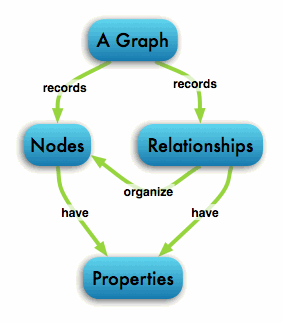
\includegraphics[width=15cm, height=10cm]{img/graphdb-propmodel}
\end{figure}

Neo4j is a NoSQL graph database that was released in 2007 and that was built and implemented with Java and Scala [28]. It implements the Property Graph Model discussed above. Neo4j is appropriate for use in production as it has ACID transaction compliance, runtime failover and cluster support.

\begin{figure}[h]
	\caption{Neo4j Example}
	\centering
	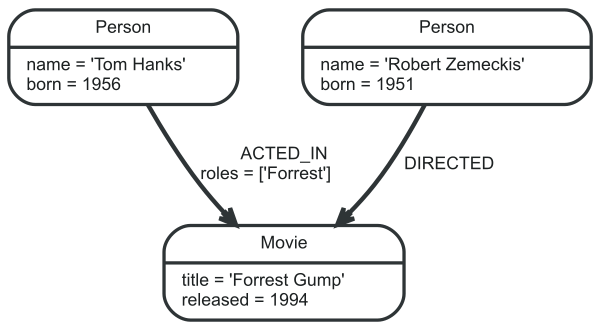
\includegraphics[width=15cm, height=10cm]{img/neo4j-example}
\end{figure}

To interact with the Neo4j database it is necessary to use the Cypher query language. Cypher is declarative query language that is inspired by SQL and it allows us to select, update, delete or insert into the Neo4j database without having to describe the “how” of doing so. The majority of Cypher queries use the following 3 key words:
\begin{itemize}
	\item MATCH – this is specifying the graph pattern you wish to match.
	\item WHERE -  this is how you add constraints to your pattern matching 
	\item RETURN – this is what you want to return.
\end{itemize}
An example of using cypher on the above Neo4j Image is as follows:
\begin{minted}{sql}
MATCH(n:Person)-[:ACTS_IN]->(n:Movie) where n.born = 1956 RETURN n
\end{minted}
The above query breaks-down as follows:
\begin{itemize}
	\item MATCH(n:Person) – this finds all nodes with the label Person
	\item -[:ACTS IN]->(n:Movie) specifies it must have a relationship with the node which has the label Movie
	\item where n.born =1956 RETURN n – where constrains the pattern to only matching a node with the property born equal to 1956 and it returns all nodes matching that pattern, so just the 1 above in the image \cite{neo4j}
\end{itemize}
\section{D3.JS}
D3 (short for data-driven documents, otherwise known as d3.js) is a library created for JavaScript that facilitates the creation of data visualisations by using common web standards such as SVG, Canvas and HTML. The creator Mike Bostock originally made the JavaScript library “Protovis”. 
However, in 2011, he unfortunately stopped the continuous development of this library and switched to improving his other creation, d3.JS., instead. D3 was created with the idea that it need not be a massive library that attempts to solve all problems and provide for every possible need. Instead, it focuses on being an efficient manipulator of the DOM by using data-driven techniques. Because it is a small library, it is much faster and allows for working with huge datasets, which allows the user to create interactive and animated visualisations.  The following code snippets show both d3s’ code efficiency as well as its usefulness with datasets. 

A standard JavaScript approach to selecting all paragraph elements is displayed below:
\begin{minted}{javascript}
var paragraphs = document.getElementsByTagName("p");
for (var i = 0; i < paragraphs.length; i++) {
var paragraph = paragraphs.item(i);
paragraph.style.setProperty("color", "white", null);
}
\end{minted}
By comparison, a basic example of D3 is displayed below: 
\begin{minted}{javascript}
d3.selectAll("p").style(colour", "white");
\end{minted}
Finally, a small example of manipulating the DOM with data is shown below:
\begin{minted}{javascript}
d3.selectAll("p")
.data([4, 8, 15, 16, 23, 42])
.style("font-size", function(d) { return d + "px"; });
\end{minted}
\section{Jquery 1.12.x}
jQuery is a free, open-source JavaScript library that allows for the manipulation of HTML elements through the scripting language JavaScriptt. It is the number one most used JavaScript library in the world [30]. jQuery was created in 2006 and is now in its third version. However, both versions 1 and 2 are still widely used. jQuery is lightweight and and fast, allowing the user to control the DOM with the use of very little code. Some of the main benefits of using jQuery include:

\begin{itemize}
	\item HTML/DOM handling and alteration.
	\item Manipulation of the CSS elements of HTML elements
	\item It has made using AJAX/JSONP much simpler to work with.
	\item It provides for both event handling and effects/animations.
	\item It has in-built cross-platform compatibility.
	\item A huge library of plugins have been created for use with jQuery.
\end{itemize}
An example of what jQuery looks like is shown below:
\begin{minted}{javascript}
$("button.continue").html("Next stop");
\end{minted}
The above code works as follows: Using the jQuery selector \textdollar, it gets hold of the button with the class "continue" and changes its HTML ( text ) to "Next stop" \cite{jquery}.
\section{Bootstrap}
Bootstrap is a HTML, JS and CSS web framework that was created by developers working for Twitter [31]. It is designed to be used for developing mobile first applications that are responsive, fast and appear neater and cleaner for UI purposes. It is only meant for use with front-end development and does not cater for other development aspects. Bootstrap has responsive CSS built-in for creating apps that scale the elements depending on the size of the screen used (e.g. desktops, tablets, smartphones). Bootstrap was created using the CSS preprocessors LESS and SASS. Bootstrap comes shipped with in-built components such as drop-downs, navigation bars, pop-overs and other regularly used web components. It also comes with jQuery plugins and is customizable to suit the users’ own designs. Some of the main advantages of using Bootstrap include: 
\begin{itemize}
	\item It has cross-browser compatibility 
	\item It is open-source
	\item Its design is consistent throughout the framework
	\item There are excellent documentation and examples provided on the Bootstrap website.
	\item Time is not wasted working on CSS when simplicity is required \cite{bootstrap}
\end{itemize}
\chapter{System Design}
This section will provide a comprehensive account of each component of the project, beginning with an outline of the overall design and architecture of the project. Following, it will discuss the process undertaken to acquire the relevant data. The Python library Scrapy was used for data extraction and Pandas library was used for the purpose of data analysis. Next, it will describe how the data was imported into the neo4j database and how the Python library “py2neo” was used to add more properties to the data. Once the data was stored as nodes, labels were then assigned to these nodes depending on their particular properties in the overall database. Following, there will be an account of how the whole application functions through the Python web framework, Flask. Finally, the design of the front end section will be described, including an example of the data visualization.
\section{System Architecture}
	\begin{figure}[h]
		\caption{System Architecture}
		\centering
		\includegraphics[width=15cm, height=4.5cm]{img/SystemArchitecture}
	\end{figure}
\pagebreak
\section{Data and Data Analysis}
\subsection{Historical Data}
While researching the results of the general elections in Ireland from 1992-2011, I came across a website called electionsireland.org [13]. This website was created in conjunction with the political analyst, Sean Donnelly. It contains the full results and statistics of each constituency in the Republic of Ireland, for every election dating back as far as the very first one in 1922. Unfortunately, the data was not freely available on the website for downloading in any format. However, given that this website contained all of the relevant data required for this project, I decided to research how to use a web scraper. As I had decided to use Python as my main programming language for this project, I found the library Scrapy. As touched upon already in my technology review, Scrapy is a Python library that does all the hard work for web crawling websites. It allows the user to specify the starting URLs as well as the selectors for the data parsing. The following is an example code snippet of what one of the three Scrapy spiders used in this project looked like:
\begin{minted}{python}
import scrapy

# this spider extracts the name and party of each person who ran 
#for election in the constituency of every election back to 1992
# note that the names are never used in this application, but 
# were downloaded at the time just in case
class ConDataSpider(scrapy.Spider):
name = "con_data"
start_urls = ['http://electionsireland.org/result.cfm?election=2016&cons=32']
#['http://electionsireland.org/result.cfm?election=1992&cons=32']
#['http://electionsireland.org/result.cfm?election=1997&cons=32']
#['http://electionsireland.org/result.cfm?election=2002&cons=32']
#['http://electionsireland.org/result.cfm?election=2007&cons=32']
#['http://electionsireland.org/result.cfm?election=2011&cons=32']


def parse(self, response):
# select the exact table the required data is in
for row in response.css('body table:nth-child(5)'): 
yield {
# get the name of the candidate
'name': row.css('tr td:nth-child(2) a::text').extract(), 
# get the party of the candidate
'party': row.css('tr td:nth-child(4) a::attr(href)').extract(), 
}

next_page = response.css('table.rhtable table:nth-child(1) a::attr(href)')
.extract()[1]
#print(next_page)
if next_page is not None: # keep going until no pages left to traverse
next_page = response.urljoin(next_page)
yield scrapy.Request(next_page, callback=self.parse)
\end{minted}
I extracted all of the relevant data that I needed from the website and stored all of it in JSON format to be used in the application. In retrospect,  using Beautiful Soup instead of Scrapy’s built-in selectors would have saved me more time, as I had to experiment a lot with the CSS selectors in order to get the exact data that I required to be parsed by the spiders. 
\subsection{Population Data}
As referenced in the methodology section, the population data came from the Central Statistics Office (CSO) and is taken from the 2011 Census section. There are two parts to the population data. The first is the general population statistics for each county. This data comes from the Table "Population by Province County or City, Detailed Marital Status, CensusYear, Sex and Age Group" on the CSO website. It produced 8 CSVS split by province and sex (e.g connaught\textunderscore females.csv). The figures are sorted by "age\textunderscore range", which is in line with how the polling data is also organized (e.g using age-ranges of 25-24, 35-49 etc.).

It was necessary to transfer text matrices from the results of the query into CSV files as the formats provided by them were unfortunately not suitable for easy Pandas manipulation. The second part of the population data was the social classes population statistics from the CSO. The table source is "Population by Socio-Economic Group, Sex, Province County or City and Year". The social classes were split into five categories in order to match the arrangement of the polling data (e.g AB, C1, DE etc). Each category was then matched into the appropriate polling data category based on a related report by Pfizer \cite{pfizer}. Again, the data formats provided by the CSO website were not suitable for use directly, so the text matrices had to be copied into CSV files.
\subsection{Data Analysis}
\subsection{Population}
\subsubsection{General Population}
The population data was sorted into CSV files by using a mixture of the Python Pandas library and Pythons’ built in CSV functionality. Ideally, refactoring the data may have made it possible to assign a reusable class for the functionality. However, in favour of saving time, I assigned a separate class for each province instead. Each class uses Pandas to extract from the population CSVs certain data, depending on the criteria provided to Pandas. 

Here is an example code snippet from one of the classes which shows how Pandas works:
\linebreak
\linebreak
\begin{minted}{python}
# put the connaught males csv into a pandas dataframe
df = pd.read_csv('app/data/population/population_data/connaughtmales.csv',
 header=None, delimiter='\t', converters={"4": int})
# append to the temp list group_list 1 - the number of people 
# that fit the criteria passed in to the dataframe
for county in self.connaught:
group_list_1 = []
group_list_1.append(df.loc[(df[1] == county) & (df[2] == 'Single')
 & (df[3] == '20 - 24 years'), 4].sum())
group_list_1.append(df.loc[(df[1] == county) & (df[2] == 'Single') &
((df[3] == '25 - 29 years') | (df[3] == '30 - 34 years')), 4].sum())
group_list_1.append(df.loc[(df[1] == county) & (df[2] == 'Single') &
((df[3] == '35 - 39 years') | (df[3] == '40 - 44 years') | (
df[3] == '45 - 49 years')), 4].sum())
group_list_1.append(df.loc[(df[1] == county) & (df[2] == 'Single') &
((df[3] == '50 - 54 years') | (df[3] == '55 - 59 years') | (
df[3] == '60 - 64 years')), 4].sum())
group_list_1.append(df.loc[(df[1] == county) & (df[2] == 'Single') &
((df[3] == '65 - 69 years') | (df[3] == '70 - 74 years') | (
df[3] == '75 - 79 years') | (df[3] == '80 - 85 years') |
(df[3] == '85 years and over')), 4].sum())
\end{minted}
Each class has three functions that return the following three lists: 1) All populations of the province, 2) The male population of the province, and 3) The female population of the province. Each list is also sorted by age group and marital status. I took an instance of each province class and looped through the population lists retrieved from these instances in order to create the CSV files. 
\pagebreak

Below is an example of a code snippet which illustrates how the loop creates rows on the CSV according to the defined characteristics of the population (e.g. ID, gender, location etc.) 
\begin{minted}{python}
# this python script is used to create CSV files that are to be imported into
# the Neo4j database usingNeo4js import functionality

connaught = ConnaughtPopulation() # create an instance of the province
# switch for males when running the script each time
#connaught.populate_female_lists() 
connaught.populate_male_lists()
#cf = connaught.get_female_lists() # switch for males
 # call the get male lists to get the data from the connaught class
cm = connaught.get_male_lists()

counties = ['Galway', 'Leitrim', 'Mayo', 'Roscommon', 'Sligo']
status = ['Single', 'Married', 'Divorced', 'Widowed'] # used in the loops

with open('app/data/province_populations_data/connaught_population_male.csv',
 'w') as csvfile: # open the relevant empty csv
 # list of the headers for the csv file
fieldnames = ['id', 'gender','location', 'martial_status'] 
writer = csv.DictWriter(csvfile, fieldnames=fieldnames)

writer.writeheader() # write the headers to the csv
count = 0 # used for creating a unique id each person to be added
for category_index, category in enumerate(cm): # switch for males
for county_index,county in enumerate(category):
for age_index, age_group in enumerate(county):
for i in range(age_group):
if age_index == 0:
writer.writerow({'id': 'cm1824' + str(count),
'gender': 'male',
'location': counties[county_index],
'martial_status': status[category_index]})
count += 1
if age_index == 1:
writer.writerow({'id': 'cm2534' + str(count),
'gender': 'male',
'location': counties[county_index],
'martial_status': status[category_index]})
count += 1
if age_index == 2:
writer.writerow({'id': 'cm3549' + str(count),
'gender': 'male',
'location': counties[county_index],
'martial_status': status[category_index]})
count += 1
if age_index == 3:
writer.writerow({'id': 'cm5064' + str(count),
'gender': 'male',
'location': counties[county_index],
'martial_status': status[category_index]})
count += 1
if age_index == 4:
writer.writerow({'id': 'cm65plus' + str(count),
'gender': 'male',
'location': counties[county_index],
'martial_status': status[category_index]})
count += 1	content...
\end{minted}
\pagebreak
\subsubsection{Social Classes}
Based on the classification system used in the Irish Times Polls [11] and the Pfizer classifications system [32], Pandas was used to extract the data from the Polling CSV files. A loop was then created to iterate through each county in each province in order to calculate what percentage of the county population belonged to each social class. The following code snippet is an example which shows what one of the social province classes looks like:
\begin{minted}{python}
import pandas as pd

# a class for calculating the % of people in each social class
class ConnaughtSocial():
def __init__(self):
self.df = 
pd.read_csv('app/data/social_class_data/connaught_social_classes.csv',
 header=None, delimiter='\t', 
 converters={"3": int}) # make a dataframe of the 4 social classes
#farmers dataframe
self.dff = 
pd.read_csv('app/data/social_class_data/connaught_farmers.csv', header=None,
 delimiter='\t', converters={"3": int})   # make a dataframe of the farmers
# counties in connaught as part of republic of ireland
self.connaught = connaught = ['Galway', 'Leitrim', 'Mayo', 'Roscommon', 'Sligo']
# list of lists of the social classes for each county, excluding the farmers 
self.connaught_social_classes = [] 
self.farmers = [] # list of number of farmers in each county
self.connaught_totals = [] # list of total number of people in each county
# list of lists of the calculated %'s of people divided into classes
self.connaught_percentages = [] 
 # fill the list of lists of populations per social classes including farmers
def populate_counties_classes(self):
for county in self.connaught:
group_list_1 = []  # ab, c1, c2, de
# sourced from  
#http://stackoverflow.com/questions/37947641/pandas-how-to-sum-columns-based-on-conditional-of-other-column-values
#ab social classes
group_list_1.append(self.df.loc[(self.df[1] == county) & (
(self.df[2] == 'Professional workers')
 | (self.df[2] == 'Managerial and technical')), 3].sum())
# c1 social class
group_list_1.append(self.df.loc[(self.df[1] == county)
 & (self.df[2] == 'Non-manual'), 3].sum())
#c2 social class
group_list_1.append(self.df.loc[(self.df[1] == county) 
& (self.df[2] == 'Skilled manual'), 3].sum())
# de social classes
de = (self.df.loc[(self.df[1] == county) & ((self.df[2] == 'Semi-skilled')
 | (self.df[2] == 'Unskilled')
| (self.df[2] == 'All other gainfully occupied and unknown')), 3].sum())

farmers = (self.dff.loc[(self.dff[2] == county), 3].sum())
# take away the farmers in this county from this social class
group_list_1.append(de - farmers) 

self.connaught_social_classes.append(group_list_1) # append ab - de
self.farmers.append(farmers) # lastly append the farmers
# make a list of the total number of people in each county
def populate_totals(self): 
for index,county in enumerate(self.connaught_social_classes):
county_total = sum(county) + self.farmers[index]
self.connaught_totals.append(county_total)
# make a list of lists of the %s of each class in each county
def set_social_percentages(self): 
for index, county in enumerate(self.connaught_social_classes):
group_list = []
for s_class in county:
group_list.append(round((s_class / self.connaught_totals[index]) * 100))
group_list.append(int(self.farmers[index] / self.connaught_totals[index] * 100))
self.connaught_percentages.append(group_list)
# return the list of lists of %s of classes in each county
def get_social_percentages(self): 
self.populate_counties_classes()
self.populate_totals()
self.set_social_percentages()
return self.connaught_percentages
\end{minted}
Notice in the populate\textunderscore counties\textunderscore classes function I had to make a provision for the Farmer social class. The number of farmers in each county were acquired by extracting data from the Central Statistics Office. This data was then stored in a separate CSV file. It was necessary to subtract the number of farmers from the DE Social Class \cite{pfizer}, so that it would match the format of the polling data. This also allowed for a more accurate representation of the population in the Republic of Ireland, as was desired.
\subsubsection{Historical}
Each election from 1992 to 2011 was analysed with the goal of calculating the percentage of seats won by each party per constituency. In the codebase, each election year was given its own class. If I had had additional time, it may have been useful to create a more generic class that could take data from any year and return the list of percentages for each party as requested.  An example of the code for these election classes is provided below: 
\begin{minted}{python}
import pandas as pd
from collections import Counter


# this calculates the average % of each party in each constituency in 2007
class Hist2007():
def __init__(self):
# scraped results from electionireland.org
self.results_2007_df = pd.read_json("results2007.json") 
# names of each constituency
self.constituencies_2007_df = pd.read_json("cons_2011_2007.json") 
# get the parties from the results
self.results_2007_unfiltered = list(self.results_2007_df['party']) 
self.constituencies_2007_uf = list(self.constituencies_2007_df['county'])  # uf stand for unflattened
self.constituencies_2007 = []
self.results_2007 = []
# seats in constituencies
self.number_of_seats = [5,5,4,4,4,3,5,3,3,3,4,4,4,3,3,3,5,5,4,
4,3,5,4,5,3,3,4,3,5,5,3,4,4,5,3,3,3,3,3,3,4,5,5]
self.historical_percentages = []

# this function gets the parties of the people elected in each constituency
def filter_results_2007(self): 
for index, const in enumerate(self.results_2007_unfiltered):
group_list = []
# depending on the number of seats in the constituency
for seat in range(self.number_of_seats[index]): 
group_list.append(const[seat])
self.results_2007.append(group_list)

def flatten_df(self):
for sublist in self.constituencies_2007_uf:
for val in sublist:
self.constituencies_2007.append(val)

def set_percentages(self):
self.filter_results_2007()
# main parties - FF, FG, SF, LB and IND. Note that anything other than these 
# 5 will be added to IND the following variables holds a list of 
# lists of the percentages of each party in each constituency
FF = []
FG = []
SF = []
LB = []
IND = []
# GP,Ind, PD, IFG, CS, WP, SP, SWP. IFF, IHA, NP
#self.number_of_seats = []
for index,constituency in enumerate(self.results_2007):
seats = self.number_of_seats[index]
# Counter counts all occurences of what it is given as a params
counts = Counter(constituency)
FF.append((counts['FF'] / seats) * 100)
FG.append((counts['FG'] / seats) * 100)
SF.append((counts['SF'] / seats) * 100)
LB.append((counts['LB'] / seats) * 100)
IND.append(((counts['Ind'] + counts['IND'] + counts['IFG'] 
+ counts['GP'] + counts['PD'] + counts['CC']
+ counts['CS'] + counts['WP'] 
+ counts['SWP'] + counts['IFF'] + counts['IHA'] + counts['NP']) / seats) * 100)

self.historical_percentages.append(FF)
self.historical_percentages.append(FG)
self.historical_percentages.append(SF)
self.historical_percentages.append(LB)
self.historical_percentages.append(IND)

def set_data(self):
#his2011 = Hist2007()
#his2011.set_data()
#self.number_of_seats = his2011.get_number_of_seats()
self.flatten_df()
self.set_percentages()

def get_data(self):
# return the percentage of wins for each party in each constituency
return self.historical_percentages 
\end{minted}
Finally, there is a class which takes the results of the above analysis for the 2011 and 2007 elections. Within this class, it is then possible to calculate the average percentage per constituency for each party. It was not possible to take election results from other years as there have been so many constituency changes over the past 10-20 years. By only focusing on the 2007 and 2011 elections, it was possible to guarantee far greater consistency and reliability across the constituencies.  Although not exhaustive, these years still provide a clear example of how this class can be applied for the purpose of this project. 
\section{Database (Neo4j)}
\subsection{Overview}
The population of the database consists of 3,140,813 people, who were all represented by individual nodes. In addition, the database also consists of five separate nodes to represent the different political parties currently active in the Republic of Ireland (i.e. Fianna Fail, Sinn Fein, Labour, Fine Gael and Independent). The independent category contains independent politicians as well as politicians that belong to more minor parties (e.g. PBP and AAA). Each of the nodes of the population have various properties. Images of the two types of population nodes used in my database, as well as an image displaying the overall list of constituency properties, are displayed below.
	\begin{figure}[h]
		\caption{Neo4j System Information}
		\centering
		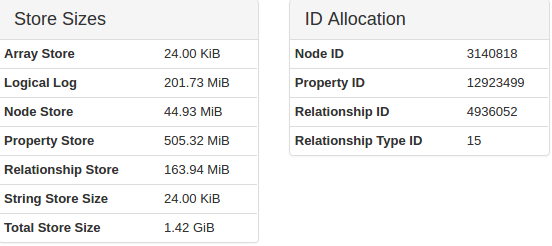
\includegraphics[width=7cm, height=3cm]{img/neo4j-monitor}
	\end{figure}
\pagebreak

The first image shows one of two types of nodes in the database. This node has the properties "marital\textunderscore status – married", "gender -female", "location – Monaghan" and a unique "id".  This node carries the following labels: "A5", "DE", "Female", "Married" and "Voter". 
\begin{figure}[h]
	\caption{Neo4j Node Example 1}
	\centering
	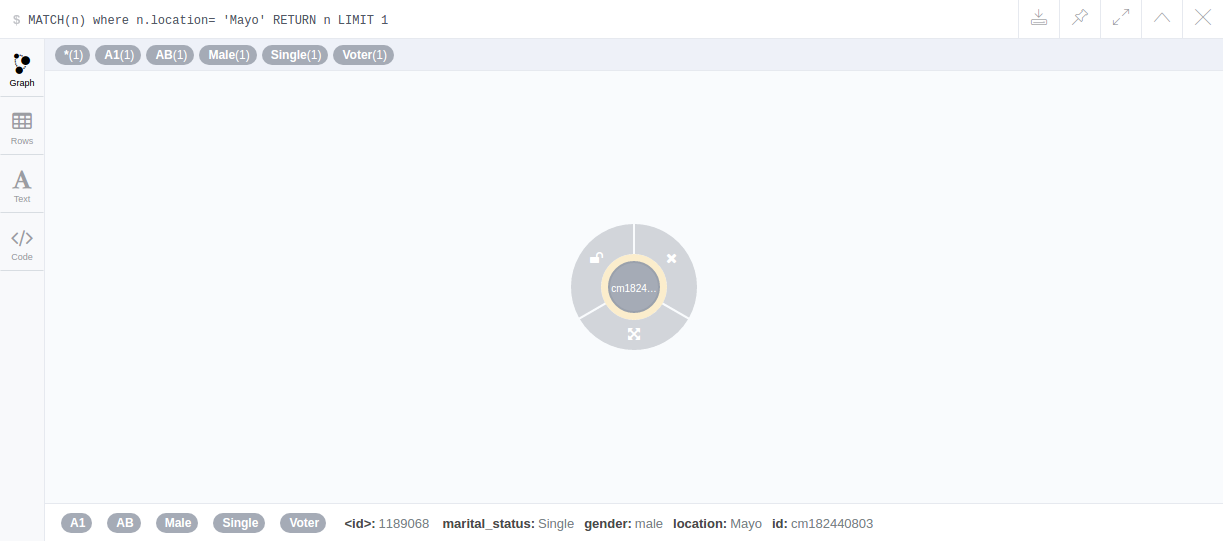
\includegraphics[width=15cm, height=10cm]{img/neo4j-noconst}
\end{figure}
\pagebreak

The second image shows the next type of  population node. This has the extra property constituency. The reason for this is that when querying the database for how many people are in a constituency, I became aware of a flaw in my original database design. Because some counties have multiple constituencies in them (e.g. Dublin had twelve of them in 2011 and 2007), it was necessary to calculate what percentage of people live in which constituency within those counties. I will describe the nature of this process in the next section (i.e. in Section 5.4.2 - Prediction). The third image displays a breakdown of the relevant constituencies. 
\begin{figure}[h]
	\caption{Neo4j Node Example 2}
	\centering
	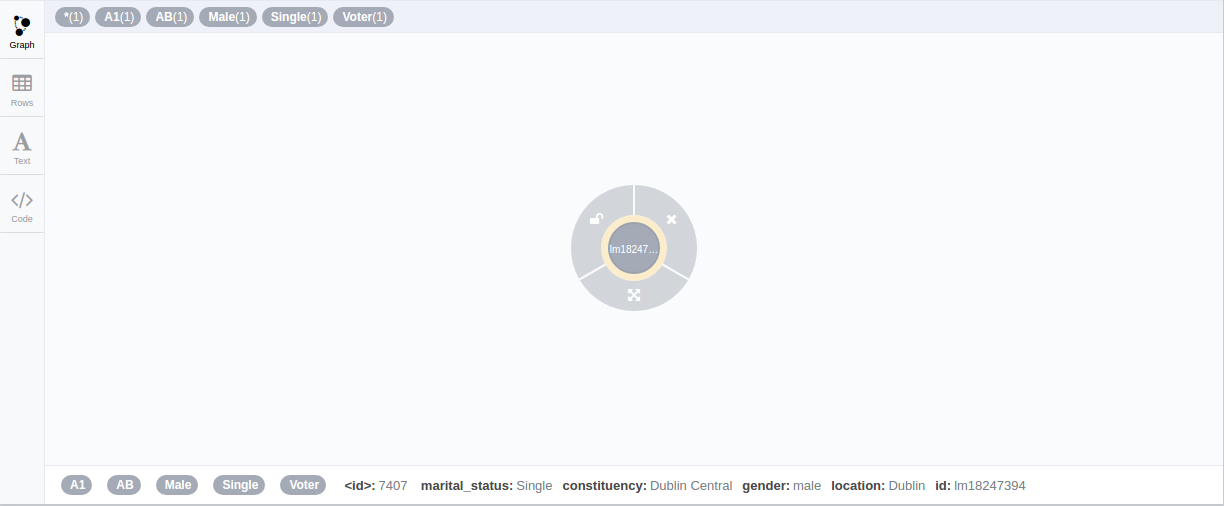
\includegraphics[width=15cm, height=10cm]{img/neo4j-const}
\end{figure}
\pagebreak

Each node has a relationship called “votes”, which dictates which party an individual will be most likely to vote for statistically, based on the prediction analysis. Along with these relationships, each node also has labels which are based on various property values (please refer to section 5.4.2. for the relevant details regarding the rationale for this decision). The image below shows the complete list of labels used in the database for this project:
\begin{figure}[h]
	\caption{Neo4j Labels}
	\centering
	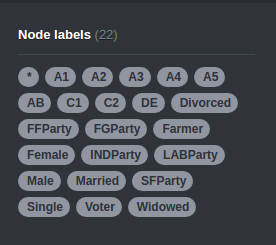
\includegraphics[width=7cm, height=3cm]{img/neo4j-labels}
\end{figure}
\linebreak

The labels A1 through A5 match the age groupings (i.e A1 = 18-24, A2 = 25-34, A3 = 35-49, A4 = 50-64 and A5 = 65+). See the Pfizer report for the Social Class listings \cite{pfizer}. As the labels were based on the properties described above, this significantly improved the speed of querying my database. 
\pagebreak

Finally, the next image illustrates an example of how the nodes of people are related to the parties within my database. 
\begin{figure}[h]
	\caption{Neo4j Relationships}
	\centering
	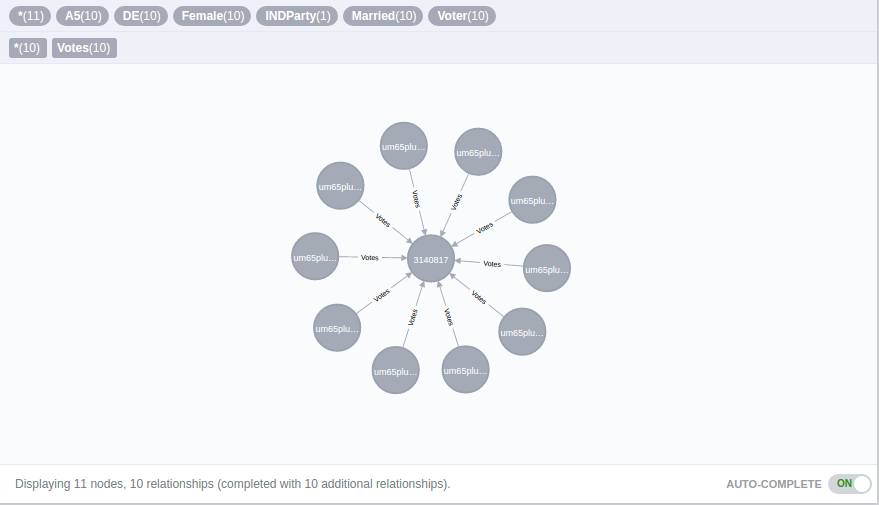
\includegraphics[width=15cm, height=10cm]{img/neo4-relationships}
\end{figure}
\pagebreak

\subsection{Database creation}
The CSV files generated from the primary population class were directly imported into the database by creating a folder in the neo4j directory called “imports”. This step was important as neo4j will not import anything unless the relevant data is stored within this specified folder. The following commands were then run on the neo4j browser console \cite{loadcsv}:
\begin{minted}{sql}
LOAD CSV WITH HEADERS FROM "file:/connaught_population_female.csv" as line
CREATE (:Voter { id: line.id, gender: line.gender, location: line.location,
 marital_status: line.martial_status})
\end{minted}
To import the files, adjustments had to be made to to the "config" file \cite{heapsize} It was necessary to increase the initial and maximum heap size settings from 512mb to 2048mb to accommodate for importing the province CSV files. For example, the Leinster province CSV contains over 900,000 rows of data to represent the population of Dublin in the database. Such a large dataset requires a greater heap size.

Finally, in order to assign labels to each node for use instead of properties, I created two types of scripts. Both of these scripts use the library py2neo. The first one is the "set\textunderscore initial\textunderscore labels" script. This script queries the database based on properties and then assigns labels to the nodes which match the queried patterns. The second script was created for assigning social class labels to each node. 
In order to do this, it was necessary to first calculate the estimated percentage of population per county present in each social class. These estimations were sourced from the social class analysis scripts which have already been described in detail above (please refer to section 5.2.3.1.2. Social Classes in the Methodology section for more information).
\pagebreak

\section{Python w/Flask}
\subsection{Overview}
The application is powered by a Python Flask framework. As touched upon briefly in the Methodology chapter, I researched work by Nicole White, a data scientist. Her work includes demonstrations of applications which combine neo4j and python using the Flask framework. One such example of a project structure created by Nicole was adapted from the Flask documentation, and served as the basis for the structure of my own application \cite{nicolewhite}.

The data folder contains all datasets used in the creation of this project. The models folder contains all scripts related to the manipulation of data and interaction with the Neo4j database. The static and templates folder hold all relevant files relating to the front-end of the application. The "\textunderscore \textunderscore init.py\textunderscore \textunderscore" file and the "views.py" file are Flask-specific and both are required for the running of the application.  The below image illustrates the Flask structure was adapted for use within the current project:

\begin{figure}[h]
	\caption{Flask Application Structure}
	\centering
	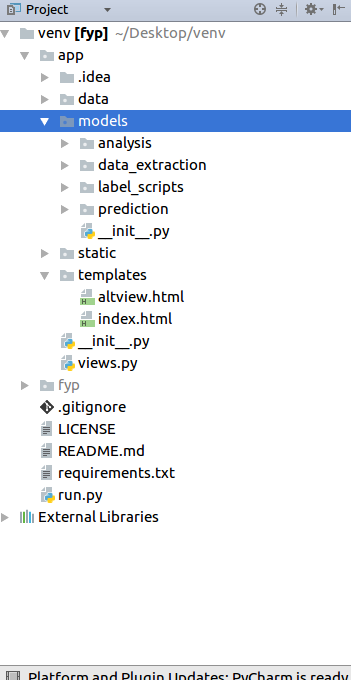
\includegraphics[width=15cm, height=10.5cm]{img/flask}
\end{figure}
\pagebreak

\subsection{Prediction Analysis}	
This section will describe the scripts created for the purpose of election forecasting. For more information regarding the research behind the chosen prediction analysis, please refer to section 3.1.3 in the Methodology section in Chapter 3. Two scripts were created, namely: 1) A probability calculator script and 2) A d’Hondt method script. 

The "probability\textunderscore calculator" script calculates the probability of voters with certain criteria (i.e. demographics) voting for a particular political party. It does this by taking all the polling data related to specified criteria and then combining this information with the historical average of the relevant constituency for each party.  It also takes into account the following two characteristics of the Republic of Ireland political system:
\begin{itemize}
	\item Some constituencies are made up of multiple counties.
	\item Some counties have multiple constituencies.
\end{itemize}
This script has one primary function that aims to process a huge amount of data as efficiently as possible (i.e. without having to create more CSV files). It uses the py2neo library to connect to the database and find voters depending on their demographic characteristics. The script then calculates their probability of voting for a particular party and sets a relationship within the database to that specified party. As Neo4j’s write performance can be quite slow, this script can take a minute or two to run depending on the matching pattern criteria specified.

The d’hondt method script uses the d’hondt method to calculate the amount of seats a party has been allocated in each constituency As there were changes to the political landscape in terms of constituency borders and the creation of new constituencies for the 2016 general election, it was necessary to make special provisions for these changes [35]. Similar to the probability calculator script, this script uses py2neo to calculate the number of votes in each party within each constituency and then applies the d’hondt method to the result to provide the estimated amount of seats per party. The data is then stored in JSON format to be used in the front-end with the d3 visualisation JavaScript library. 
\pagebreak

\section{Front-End}
The below images display the two views created for the front-end of this application. The first one shows two interactive maps of Ireland. The maps were created with the d3 v2 visualisation functionality, which made it possible to display maps of the Republic of Ireland. The reason for using v2 instead of the most recently released version (i.e. v4) is that v2 facilitated the map creation process more easily. V4 appeared to be more complicated to use in order to perform this task. Hence, I decided to opt for v2 in the end. 
The codebase for the front-end has been adapted from another project I discovered online using the map functionality of d3 \cite{tax}. The data for the two maps is stored in two separate JSON files, one holding the predictions and the other holding the actual results of the 2016 general election in Ireland. The three images below show the first of the two available views for the application. It has two maps of Ireland, the first map holding the prediction data and the second map holding the actual results and the data displayed between them. 

\begin{figure}[h]
	\caption{Front-End View Example 1}
	\centering
	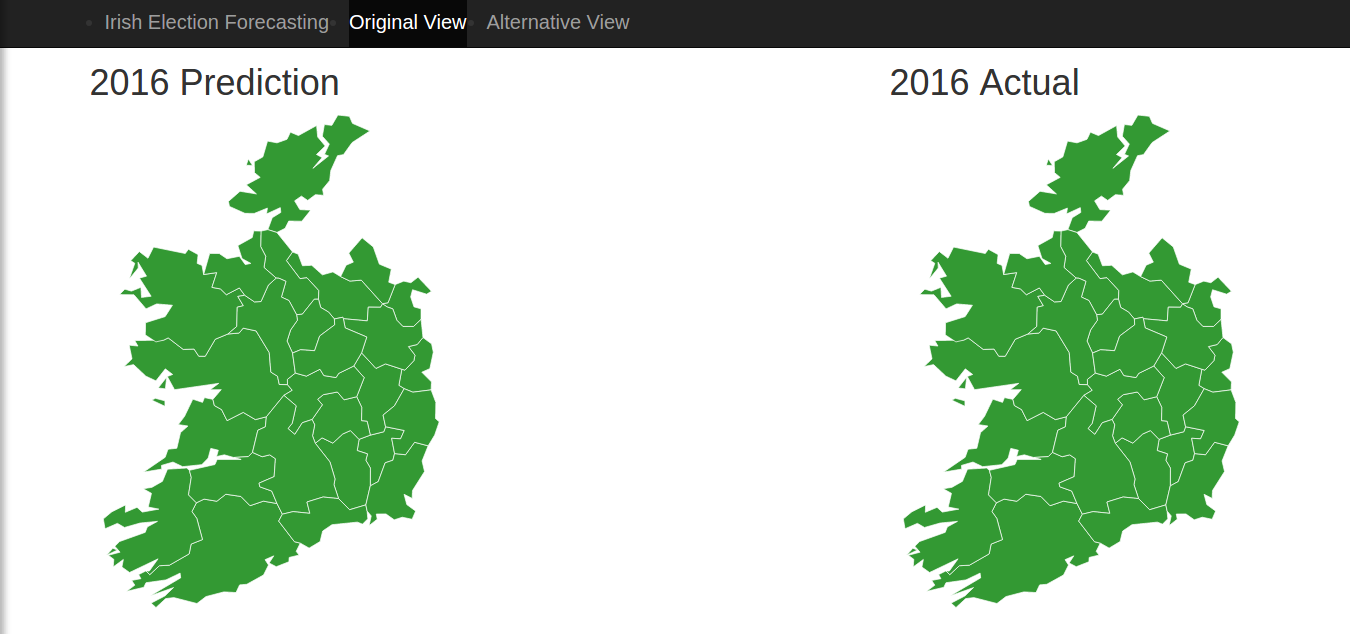
\includegraphics[width=10cm, height=5cm]{img/view1}
\end{figure}
\begin{figure}[h]
	\caption{Front-End View Example 2}
	\centering
	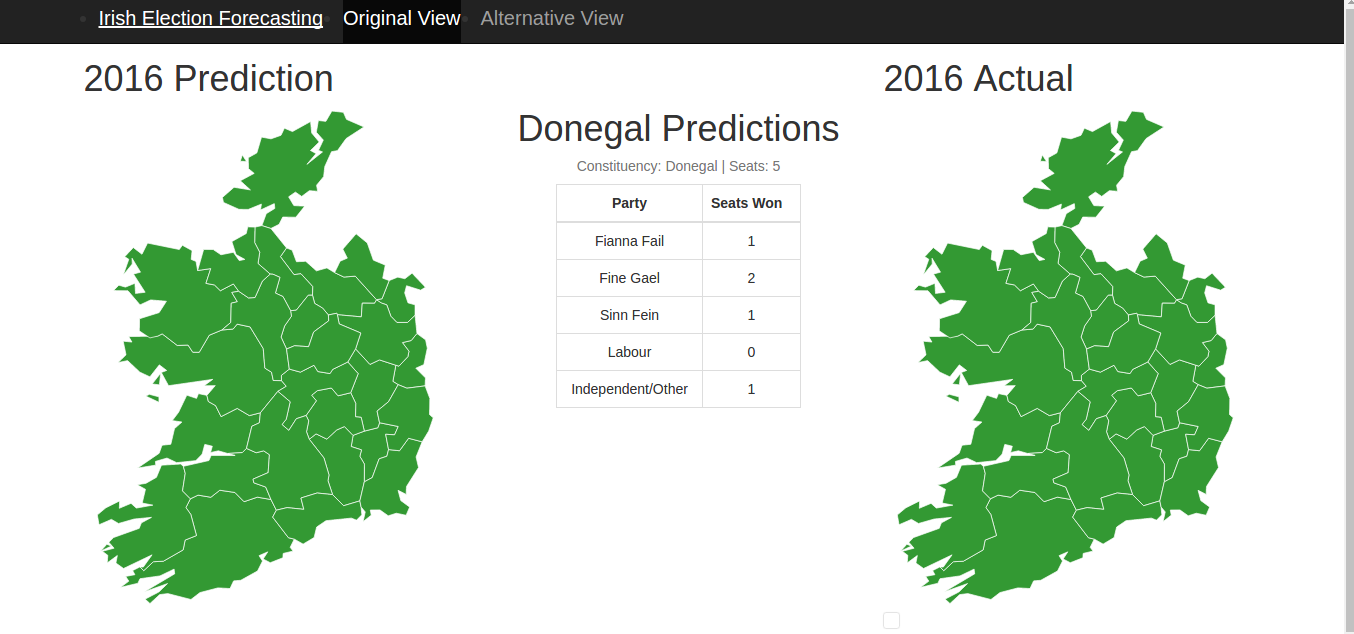
\includegraphics[width=10cm, height=5cm]{img/view1part2}
\end{figure}
\begin{figure}[h]
	\caption{Front-End View Example 3}
	\centering
	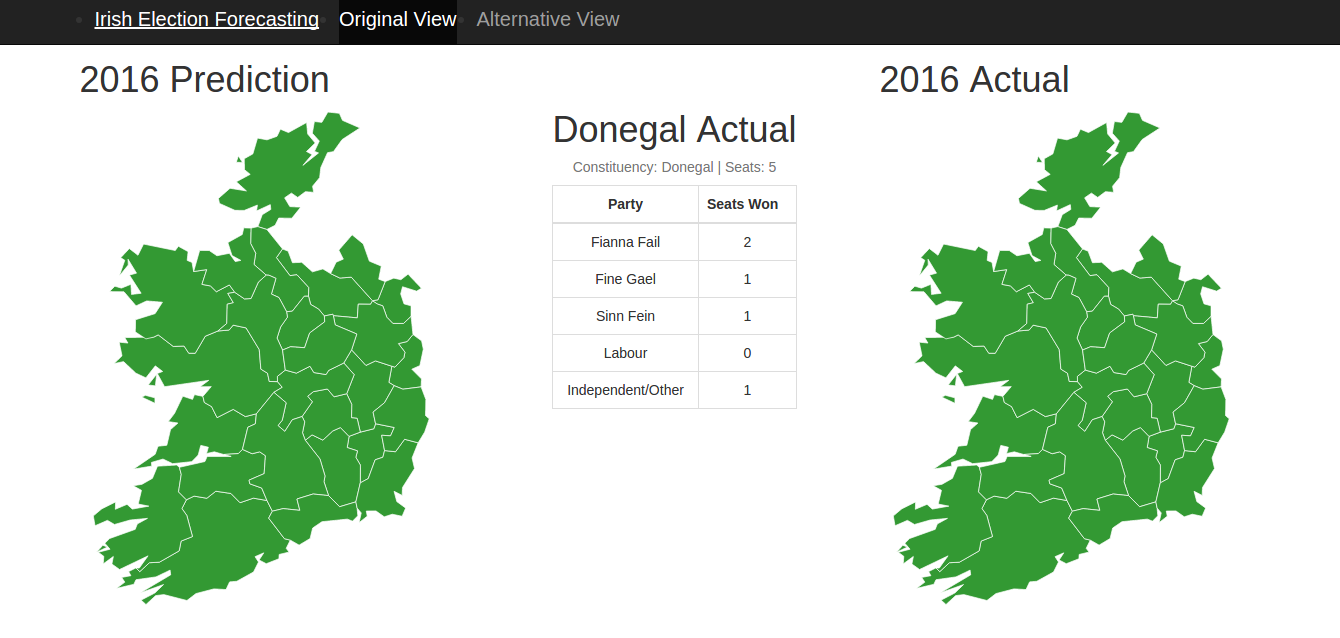
\includegraphics[width=10cm, height=5cm]{img/view1part3}
\end{figure}

\pagebreak

The next two images display an alternative view available for the application. As can be seen, this view allows the the user to compare the predictions and the actual results side-by-side as both datasets are stored on the one map. 
\begin{figure}[h]
	\caption{Front-End View Example 4}
	\centering
	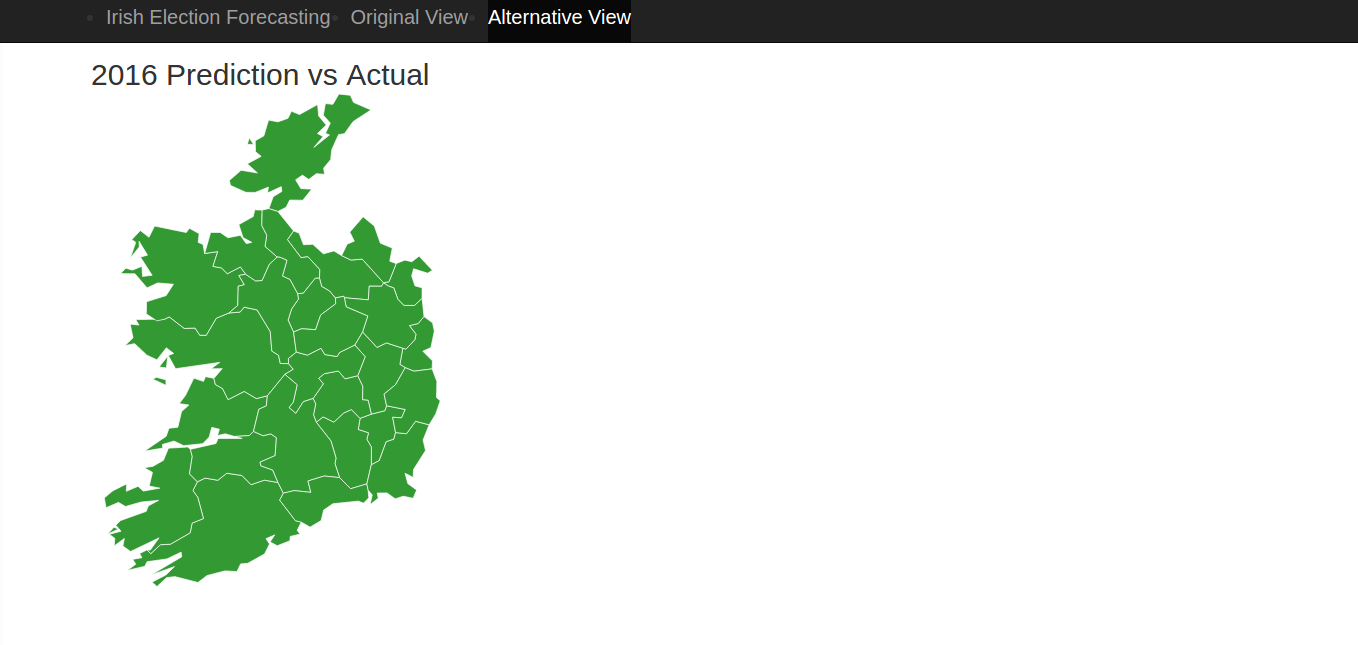
\includegraphics[width=10cm, height=5cm]{img/view2part1}
\end{figure}
\begin{figure}[h]
	\caption{Front-End View Example 5}
	\centering
	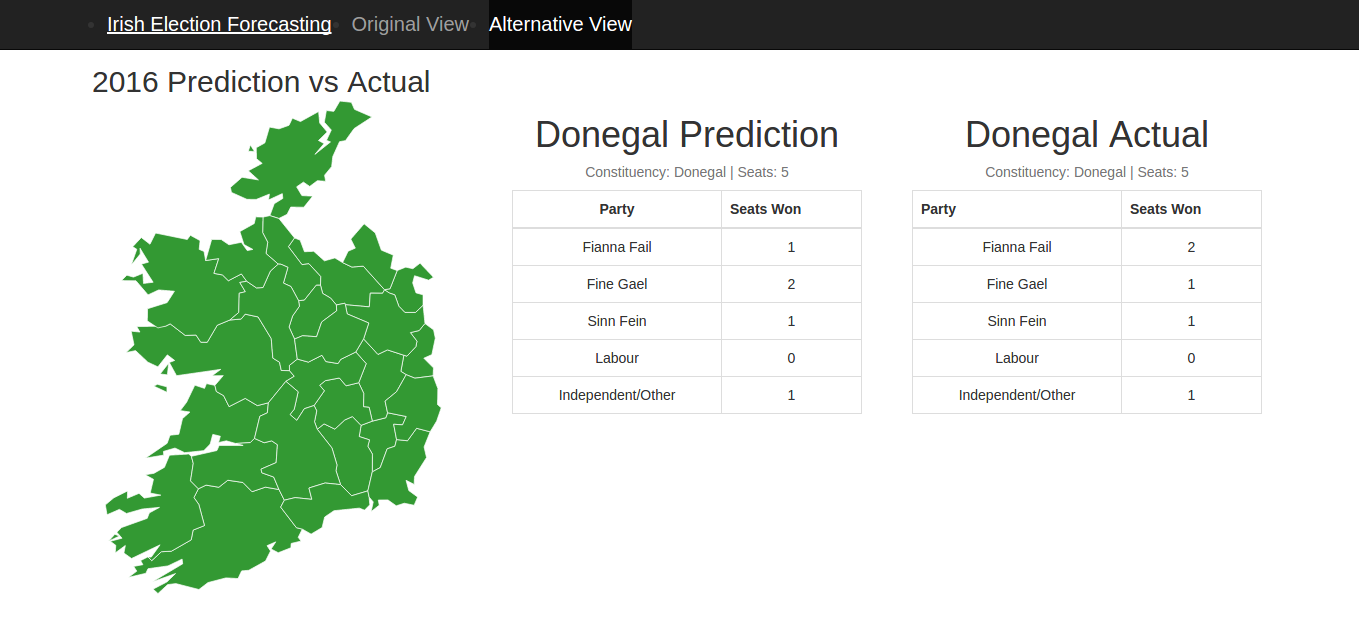
\includegraphics[width=10cm, height=5cm]{img/view2part2}
\end{figure}
\chapter{System Evaluation}
This section will discuss the outcomes of this project, with a view to evaluating how the goals of the project have been achieved according to my original objectives. It will also highlight any relevant limitations, along with providing recommendations for any future investigations in this context.
\section{Objectives vs Outcomes}
The purpose of this project was to create an example of how an application could be built and data analytics used to predict the results of a general election in Ireland. Specifically, I aimed to predict the results of the 2016 election as an example of how such an application could be designed. It was easily possible to benchmark the accuracy of my application by simply comparing my prediction outcomes with the actual results for the 2016 general election. As the map shows, these predictions are not entirely accurate. There a number of reasons for this which I will outline as limitations in section 6.2. I will also suggest various recommendations which may help to overcome these limitations for any future investigations in my conclusion section.  

Nevertheless, this application also carries a number of strengths in its evaluation. Firstly, it is functional and it therefore fulfils the main objective of the project simply by illustrating proof of concept. This has been achieved through the creation of a Python Flask framework application with a Neo4j database and of a front-end using d3.JS. This provides a working template for all future investigations in this context.  Secondary, in terms of robustness, I feel that the project is set up in a way that means that adjustments to the general prediction design can be easily implemented by editing the probability calculator script. An expert in political science or data analytics could potentially put an alternative prediction design into that class and then run the program again to obtain more accurate results in future.  Thirdly, although the front-end of my application may appear somewhat basic visually, it is also user-friendly and sufficiently interactive to serve its intended purpose. 
\section{Limitations}
The three main limitations which emerged throughout the creation process for this application will be discussed in this section. They can be roughly summarized as follows: 1. A lack of accuracy in terms of the method used for prediction, 2. The time required to run each script and 3. A lack of inbuilt diverse functionality for the front-end.
   
Firstly, the method used for prediction in this application is a very basic interpretation of ideas taken from Nate Silver (creator of fivethirtyeight.com) and Dr. Adrian Kavanagh, an Irish political analyst. 
The area of predictive analytics in terms of computer science is arguably a more complex field as it requires substantial additional expertise in the area of statistics and political science. Furthermore, it would have been beyond the allotted time-frame and scope of this particular project to attempt a more complex model. Therefore, while never being likely to be entirely accurate in its method, the more basic design used served as a justified compromise in achieving the competing goals of this project. 

Secondly, the time taken to run each script was slowed down by the use of py2neo for writing to database. In hindsight, it would have been more efficient to use Neo4j import tools to import all data into the database directly. This would have also likely allowed the final script to run slightly faster. Using py2neo to query from the database only may also have helped in this regard.

Thirdly, although never part of my core objectives, it now seems wasteful that the project was not designed with more diverse options for functionality in the front-end. For example, it could have been useful if there had been an in-built database search function for the user to explore any particular population characteristics as desired. However, time was unfortunately another constraint in this regard again. 
\chapter{Conclusion}
I started this project with no experience of any of the technologies used in the process of its development. I had never before attempted a project requiring the application of data analytics and prediction analysis techniques. I therefore now feel that I have learned a huge and diverse amount in a relatively short space of time over the past few months. All in all, I feel that this learning is reflected both in my final application as well as in this dissertation outlining the rationale behind each step of the process.  

Election forecasting is becoming of increasing interest within the field of computer science. This is due in part to the increased availability of relevant population data, but also because of the increasing power of processors for coping with increasing computational complexity. The overall goal of this project was to create a web application specifically for election forecasting in an Irish-setting, based on the results of previous elections and polling data. 

To recap, the objectives I set out in order to achieve this goal were as follows: 1) To create a database for the republic of Ireland's electorate, including future possible electorate members, 2) To create a model which could predict the results of the 2016 general election and illustrate how this can be implemented in practice and 3) To create interactive maps of Ireland which would display the predicted or actual results, depending on which map was clicked. 

As described above, the project has a number of strengths in the evaluation of its application. It provides a working template for election forecasting in a Irish setting, as well as an example front-end platform which could be used for data visualization in this context. Furthermore, it has compiled a comprehensive database concerning the demographic characteristics of the 2011 census data. 
I have also outlined a number of barriers faced in achieving the goals of this project, including the time constraints and my lack of expertise in the area of statistical analysis and political science.
 
However, insights can be gained from these limitations for future developers who are likely to encounter similar challenges in attempting a more cohesive prediction model. In the next and final section, I will outline some recommendations which I think may be helpful to bear in mind for any future investigations in this context.

\section{Recommendations}
Firstly, the scope which there could be to develop a more comprehensive model with greater accuracy could be greatly improved with a more diverse team of developers associated with varying backgrounds of expertise. An example of such a team could include an expert in political science, an expert in data analytics and software developers with varying levels of experience. This would allow for the use of a more complex statistical prediction model in this context.

Secondly, Neo4j is one of perhaps the most powerful applications currently available for creating multiple relationships between data as it is based on graph theory. Although it was not possible to display its full potential in the current project, it is important to highlight this point for future developers interested in this area. 

Thirdly, when importing data, it is most efficient to use Neo4j’s import tools in order to import data into the database directly. Compared to using a REST interface such as py2neo, this is a much faster method.

Fourthly, there is huge potential when building this type of application to leave more scope for the diversity of the front-end functionality. I think that the idea of auto-generating graphs and maps based on user input by combining py2eno and d3 would make this an interesting additional feature for the application. For example, this could allow the user to potentially search for different demographic characteristics of the general population from the 2011 census.

Finally, the idea of this project was originally inspired by the provisional release of the 2016 census 2016. Upon further investigation, it became apparent that this dataset was too incomplete for use in the current project. However, it is likely that this dataset will be fully released in the near future. This dataset may offer an exciting opportunity to provide an accessible representation of the current demographic breakdown of the Irish population in an interactive map format. Furthermore, it will also provide an up-to-date dataset for use in any future investigations concerning election forecasting in an Irish setting. 

\chapter{Appendix}
\begin{itemize}
	\item https://github.com/DevEMCN/Irish-Election-Forecasting---FYP
	
	\item https://github.com/DevEMCN/final-year-project-template
\end{itemize}
